\chapter{
Basic Statistical Concepts
}
\markboth{Modeling}{}
\label{chapt.modeling}


\vspace{.3in}

In the previous chapter we described basic concepts of
capture-recapture methods, and explained the limitations of
non-spatial models. We emphasized the advantages of
spatial capture-recapture methods, but we assumed very little
statistical knowledge. Although it is critical to understand the
non-technical motivation for this broad class of models, it is
impossible to fully appreciate them, and apply them to real data,
without a solid grasp of the fundamentals of statistical
inference.

In this chapter, we present a brief primer on key
statistical concepts that are referenced throughout the remainder of
this book. For some readers, this material will be familiar,
perhaps even elementary, and thus you may want to skip to the next
chapter. However, our experience is that many basic statistics courses
taken by ecologists do not emphasize the important subjects covered in
this chapter. Instead, there seems to be much attention paid to
minor details such as computing the number of degrees of freedom in
various $F$-tests, which, although useful in some contexts, do not
provide the basis for drawing conclusions from data and evaulating
scientific hypotheses---the objectives of statistical inference.

In addition to being basic, all of the material in the
beginning of this chapter is explained in numerous other
texts. %\citet{casella_burger:2002}
Excellent technical treatments that emphasize ecological
problems are given by
\citet{williams_etal:2002}, \citet{royle_dorazio:2008} and
\citet{link_barker:2010}. A very accessible introduction to some of the
topics covered in this chapter is presented in Chapter 3 of
\citet{mackenzie_etal:2006}. With all these excellent references, one
might wonder why we bother rehashing these concepts here. Our motivation is
two-fold: first, we wish to develop this material using examples
relevant to spatial capture-recapture, and second, we find that most
introductory texts are not accompanied by code that can
assist the novice. We therefore attempt to present simple \R~code
throughout this chapter so that those who struggle with equations and
mathmatical notation can learn by doing. As mentioned in the Preface,
we rely on \R~because it provides tremendous flexibility for analyzing
data and because it is free. We do not, however, try to explain how to
use \R~because there are so many good references already, inluding
\citet{venables_ripley:2002,bolker:2008,venables_etal:2012}.

Following our introduction to basic statistical concepts, we lay out our
philosophy of modeling ecological data, including spatial
capture-recapture data. We also introduce hierarchical
models, and discuss why they are relevant to so many problems in
ecology. Finally, we address the common concerns levied against the
hierarchical modeler, \emph{e.g.} assumptions are bad.

\section{Random Variables and Probability Distributions}

\subsection{Stochasticity in ecology}

{\bf XXXXX We need to talk about use of X vs use of x. The usage here
  is correct but we don't do this throughout the book XXXXX}

Few ecological processes can be described using purely deterministic
models, and thus we need a formal method for drawing conclusions from data while
acknowledging uncertainty. This is the role of statistical inference,
which is founded on the laws of probability. For our purposes, it
suffices to be familiar with a small number of concepts from
probability theory. The most important of which is the concept of a random
variable, say $X$. We wish to know the probability that a realization
of $X$ takes on some value $x$, %. That is, we want to be able to describe
$\text{Pr}(X=x)$, or perhaps the probability that $x$ lies within some
range of valuse. An approach for acheiving such goals is to develop a
statistical model for $X$ and then estimate the parameters of the
model by fitting it to data collected during an experiment.

To clarify the concept of a random variable, let $X$ be the number of
American shad (\emph{Alosa sapidissima}) caught after $K=20$ casts at
the shad hole on Deerfield River in Massachusetts. Suppose that
we had a good day and caught $x=7$ fish. If there were no random
variation at play, we would say that the probability of catching a
fish $p$ is exactly 0.35 and we would always catch 7 shad after 20
casts. In other words, our deterministic model is $x =
0.35\times K$. In reality, however, we can be pretty sure that this
deterministic model would not be very good. Even if we knew for
certain $p \equiv 0.35$, we would expect some variation in the number
of fish caught on repeated fishing outings. To describe this
variation, we need a model that acknowledges uncertainty (i.e.,
stochasticity), and specifically we need a model that describes the
probability of catching $x$ fish given $K$ and $p$,
$\text{Pr}(X=x|K,p)$.

To specify a model for $\text{Pr}(X=x|K,p)$ we need a specific type of
function known as a probability mass function (pmf). Or, in the case
where $X$ is a continuous random variable, we need a probability density function
(pdf). We will generically refer to these as probability distributions.
Statisticians make things easier for themselves,
and more complicated for everyone else, by using different notation
for probability distributions. Sometimes you will see
$\text{Pr}(X=x|K,p)$ expressed as $f(x|K,p)$ or $f(x; K,p)$ or
$p(x|K,p)$ or $\pi(x|K,p)$ or $\mathbb{P}(x|K,p)$ or $[x|K,p]$ or even
just $[x]$! Just remember that these expressions all have the same
meaning---they are all probability distributions which tell us the
probability of observing any possible realization of the random
variable $X$.

In this book, we will use bracket notation (the last two
examples above) to represent arbitrary probability distributions. The
key thing to remember when you see $[x]$ is that we are referring to
the probability distribution for the random variable $x$, which could
be anything: Poisson, Gaussian, beta, etc... When
we wish to be specific about the probability distribution, we will do
so in one of two ways, one precise and one symbolic. Before explaining
these two options, let's choose a specific distribution as a model for
the data in our example. In this case, the natural distribution for
$[x|K,p]$ is the binomial. The precise representation of this
distribution will be shown as:
\begin{equation}
  [x|K,p] = %\text{Bin}(K,p) =
             \binom{x}{K}p^x(1-p)^{K-x}.
  \label{modeling.eq.bin}
\end{equation}
The right-hand side of this equation is the binomial pmf (described in
more detail in Sec.~\ref{sec.modeling.distributions}), and plugging in
values for the parameters $K$, and $p$ will return the probability of
observing $x$. This is precise, but cumbersome to write repetitively,
and it may make the eyes glaze over when seen too often. Thus, we will
often simplify Eq.~\ref{modeling.eq.bin} using the symbolic notation:
{\bf XXXXX below -- little x or big X?? XXXXX}
\begin{equation}
  x \sim \text{Binomial}(K, p)
  \label{modeling.eq.binsym}
\end{equation}
%In cases where $x$ is continuous, we refer to
%$[x]$ as a probability density functions (pdf), or when
%$x$ is discrete, we call $[x]$ a probability mass functions (pmf).
%In parametric inference, we assume a particular distribution for $x$, which in
%this case would naturally be the binomial distribution, $x \sim
%\text{Binomial}(K, p)$, where $p$ is the
%probability of catching a shad on a particular cast and $K$ is the
%binomial size parameter.
The ``$\sim$'' symbol is meant to represent a stochastic relationship, and
can be read ``is distributed as.''
%We  will use this notation to complement the bracket notation, which will
%be reserved for generic probability distributions. Thus, we could
%refer to the distribution of $x$ as
%$[x]$, with possible options being $x \sim \text{Binomial}(K,p)$ or $x \sim
%\text{Poisson}(Kp)$.
Another reason for using this notation is that
it resembles the syntax of the \bugs~language, which we will
frequently use to conduct Bayesian inference.

Note that once we choose a probability distribution, we have chosen a
model. In our example, we have specified our model as $x \sim
\text{Bin}(K,p)$, and because we are assuming that the parameters are
known, we can make probability statments about future
outcomes. Continuing with our fish example, we might want to know what
the probability of catching $x=7$ again on a future fishing outing
assuming that we know $p=0.35$. Evaluating the binomial pmf returns a
probability of 0.18, as show using this bit of \R~code:
\begin{verbatim}
> dbinom(7, 20, 0.35)
[1] 0.1844012
\end{verbatim}
By definition, the pmf allows us to evaluate the probability of observing
any $x$ given $K=20$ and $p=.35$, thus the distribution can be visualed
by can be visualized by evaluating it for all values of $x$ that have
non-negligible probabilities, as can be easily done in \R:
\begin{verbatim}
plot(0:20, dbinom(0:20, 20, 0.35), type="h", ylab="Probability",
     xlab="Number of shad caught (x)")
\end{verbatim}
the result of which is shown in Fig.\ref{modeling.fig.bin} with some extra details.
\begin{figure}[ht!]
  \centering
  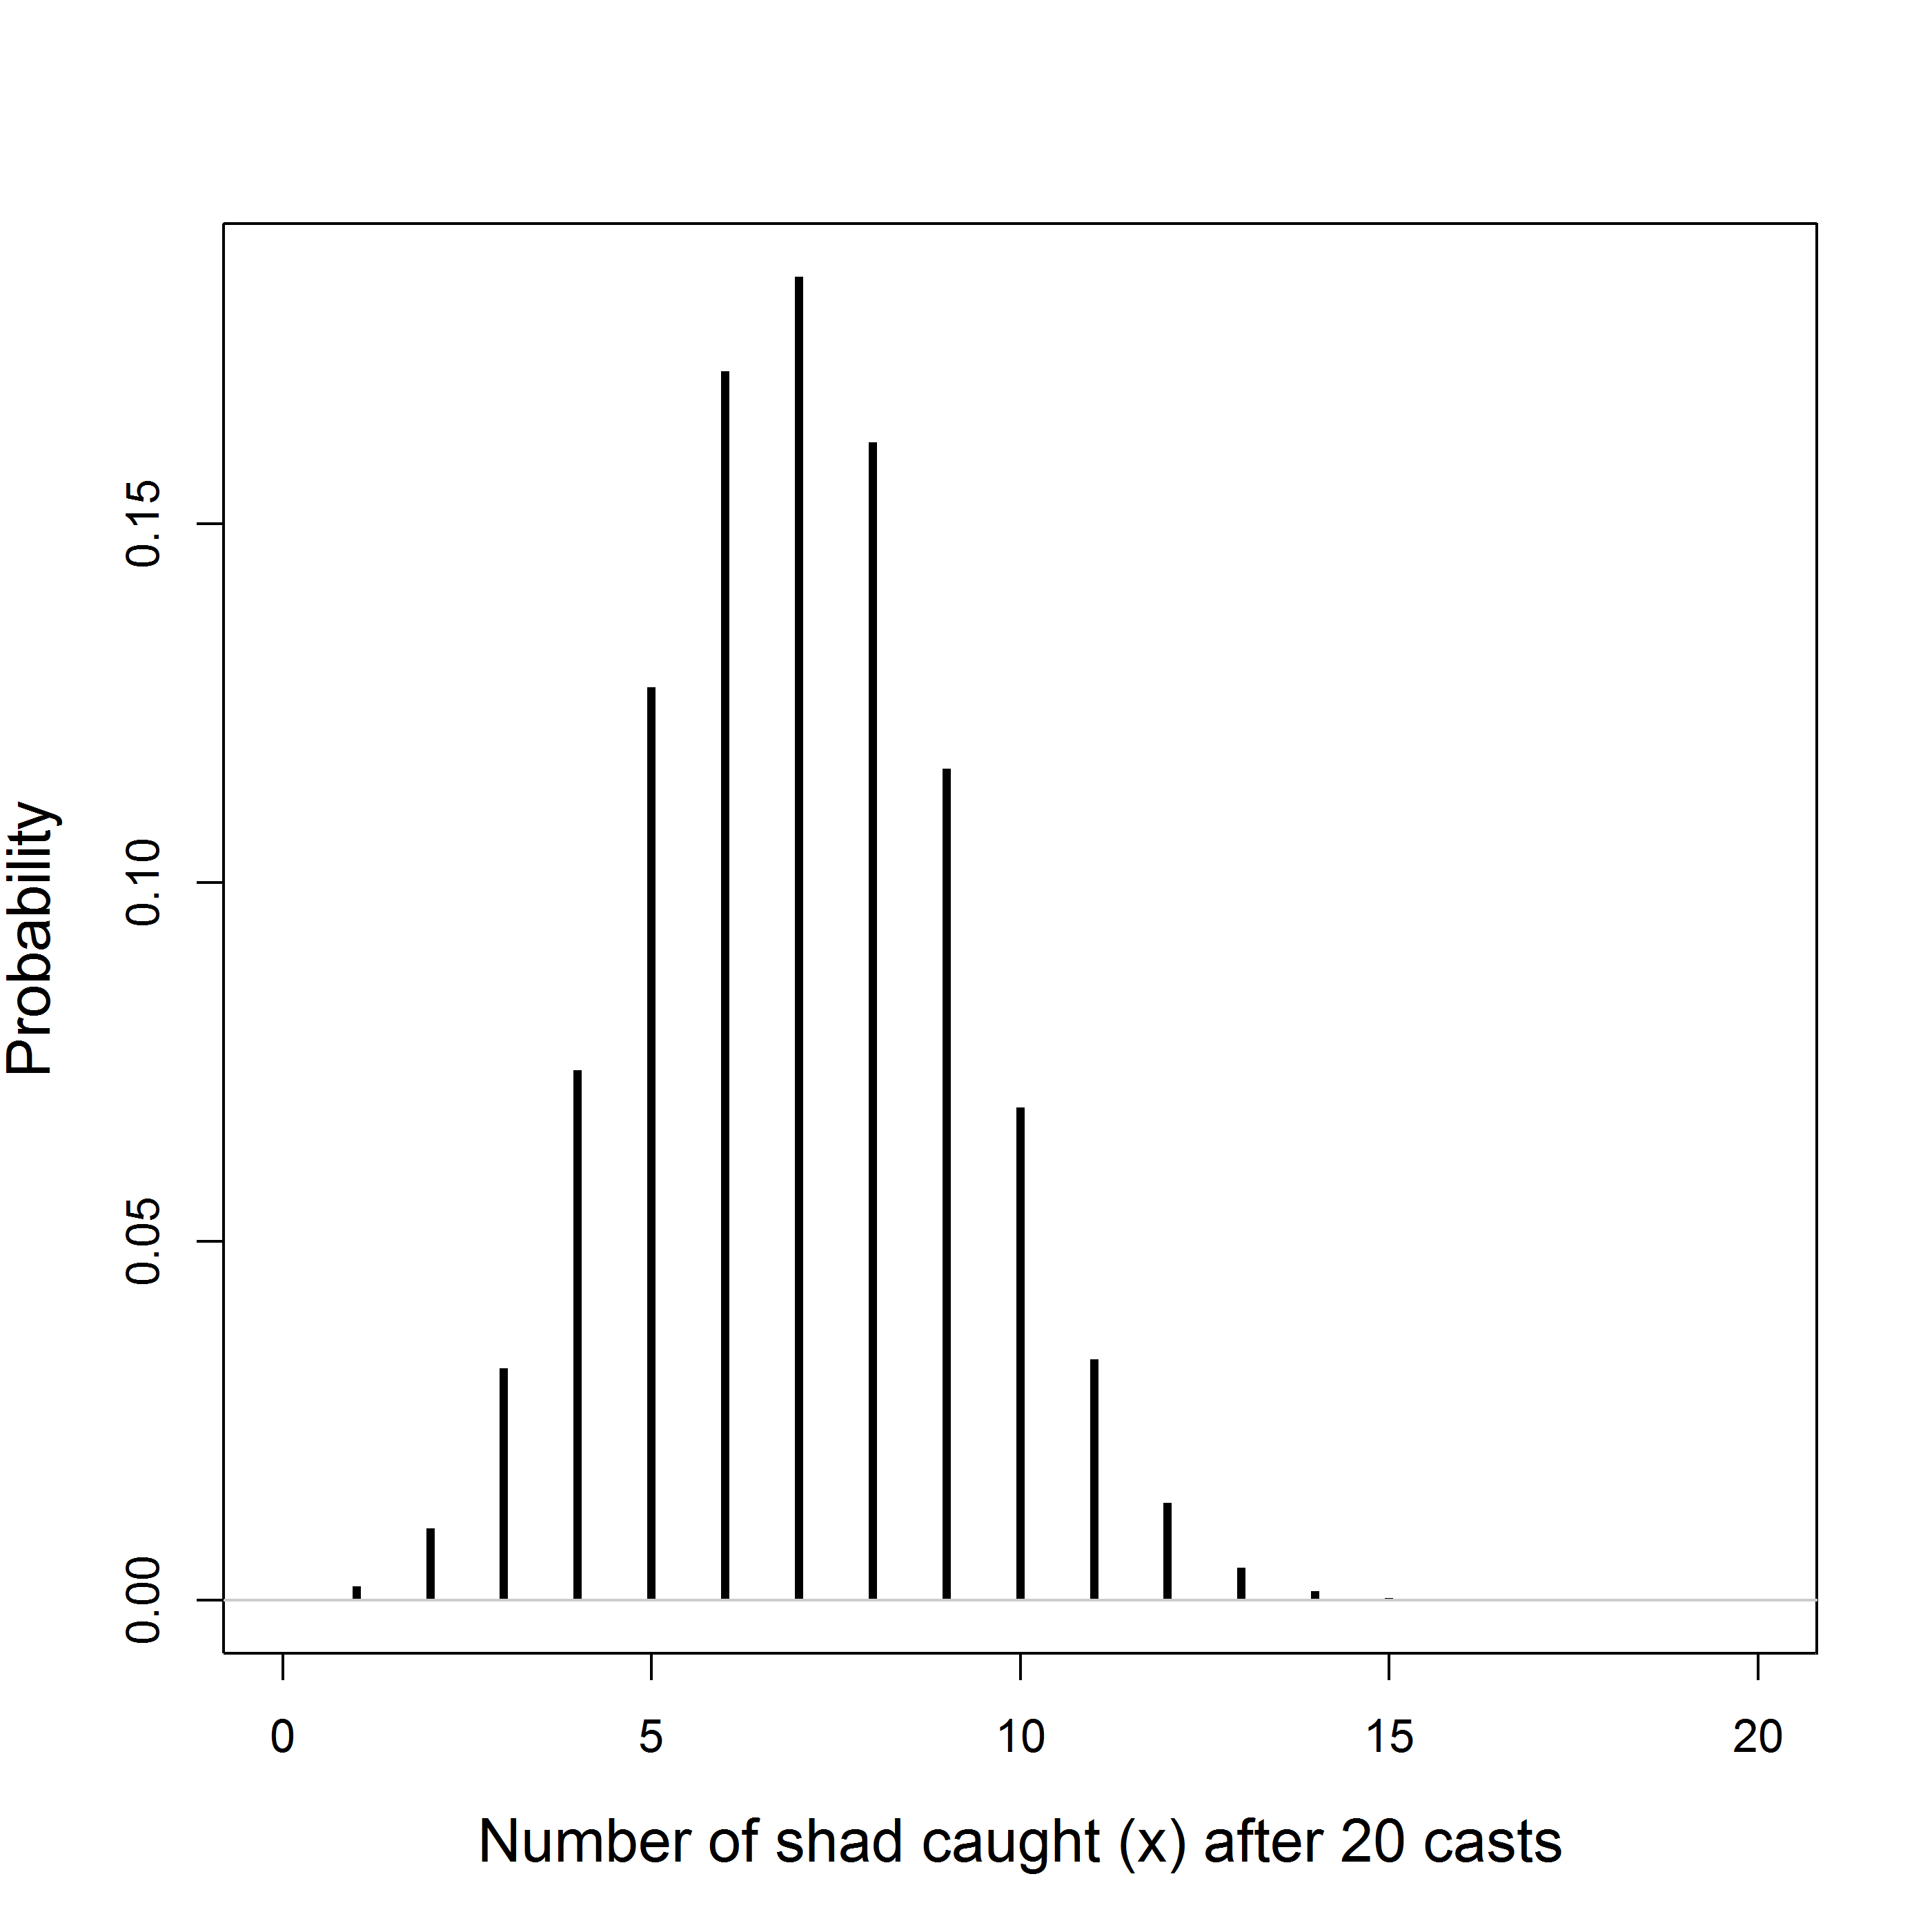
\includegraphics[width=4in,height=4in]{Ch1b/figs/bin}
\caption{The binomial probability mass function with $N=20$ and
  $p=0.35$. }
\label{modeling.fig.bin}
\end{figure}

The purpose of this little example is to show that once we specify a
model for the random variable(s) being studied, we can begin drawing
conclusions, i.e. making inferences, about the processes of interest,
even in the face of uncertainty.
Probability distributions are
essential to this process, and thus we need to
understand them in some more depth.


%%%% Add support??
\begin{table}[t!]
  \small
  \caption{Common probability density functions (pdfs) and probability
    mass functions (pmfs) used throughout this book.}
  \begin{tabular}[t]{lcccc}
    \hline
    Distribution & Notation & pmf or pmf & Mean & Variance \\
    \hline
    \multicolumn{5}{c}{Discrete random variables} \\
    Poisson & $x \sim \text{Pois}(\lambda)$ &
    $\exp(-\lambda )\lambda^x/x!$ & $\lambda$ & $\lambda$ \\
    Bernoulli & $x \sim \text{Bern}(p)$ & $p^x(1-p)^{1-x}$ & $p$ &
    $p(1-p)$  \\
    Binomial & x $\sim \text{Bin}(N, p)$ & $\binom{x}{N}p^x(1-p)^{N-x}$
    & $Np$ & $Np(1-p)$  \\
    Multinomial & $\mathbf{x} \sim \text{Multinom}(N, \bm{\pi})$ &
    $\binom{N}{x_1 \cdots x_k}\pi_1^{x_1} \cdots \pi_k^{x_k}$ & $N\pi_k$
    & $N\pi_k(1-\pi_k)$ \\
    \multicolumn{5}{c}{Continuous random variables} \\
    Normal & $x \sim \text{N}(\mu, \sigma^2)$ & $\frac{1}{\sigma\sqrt{2\pi}}
      \exp(-\frac{(x-\mu)^2}{2\sigma^2})$ & $\mu$ & $\sigma^2$  \\
    Uniform & $x \sim \text{Unif}(a, b)$ & $1/(b-a)$ & $(a+b)/2$ &
    $(b-a)^2/12$  \\
%    2D-Uniform & $\mathbf{x} \sim \text{Unif}(\mathcal{S})$ & $1/A(\mathcal{S})$ & &  \\
    Beta & $x \sim \text{Beta}(a, b)$ &
    $\frac{\Gamma(a+b)}{\Gamma(a)+\Gamma(b)}x^{a-1}
    (1-x)^{b-1}$ & $a/(a+b)$ & $\frac{ab}{(a+b)^2(a+b+1)}$ \\
    Gamma & $x \sim \text{Gamma}(a,b)$ &
    $\frac{b^a}{\Gamma(a)}x^{a-1}\exp(-bx)$ & $a/b$ & $a/b^2$  \\
    \hline
  \end{tabular}
  \label{modeling.tab.pdfs}
\end{table}




\subsection{Properties of Probability Distributions}

A pdf or a pfm is a function like any other function
%Probability distributions are functions like any other functions
in the sense that it has one or more arguments whose values determine
the result(s) of the function. However, probability functions have a few
properties that distinguish them from other functions.
The first is that the function
must be non-negative for all possible values of the random variable
$X$, i.e. $[x] \geq 0$. The second requirement is that the integral of
a pdf must be unity, $\int_{-\infty}^{\infty} [x] = 1$, and similarly
for a pmf, the summation over all possible values is unity, $\sum_x [x]
= 1$. The following \R~code demonstrates
this for the normal and binomial distributions:
\begin{verbatim}
> integrate(dnorm, -Inf, Inf, mean=0, sd=1)$value
[1] 1
> sum(dbinom(0:5, size=5, p=0.1))
[1] 1
\end{verbatim}
This requirement is important to remember when one must develop a
non-standard probability distribution. For example, in Chapt.
~\ref{chapt.state-space} and \ref{chapt.rsf},
we work with a resource selection function (RSF) whose probability
density function is not one that is pre-defined in software packages
such as \R~or \bugs.

Another feature of probability distributions is that they can be used
to compute important summaries of random variables. The two most
important summaries are the expected value, $\mathbb{E}(X)$,
and the variance $\text{Var}(X)$. The expected value
can be thought of as the average
of a very large sample from the specified distribution. For
example, a mindless way of approximating the expected values of a binomial
distribution with $K=20$ trials and $p=0.35$ can be implemented in \R~using:
\begin{verbatim}
> mean(rbinom(10000, 20, 0.3))
[1] 6.9865
\end{verbatim}
For most probability distributions used in this book, the expected
values are known exactly, as shown in Table~\ref{stat.tab.pdfs}, and
thus we don't need to resort to such Monte Carlo approximations. For instance, the
expected value of the binomial distribution is $\mathbb{E}(x) = Kp =
20 \times 0.35 = 7$. In this case, it happens to take an integer
value, but this is not a necessary condition, even for discrete random
variables.

A more formal definition of an expected value is the average of all
possible values of the random variable, weighted by their
probabilities. For continuous random variables, this weighted average
is found by integration: {\bf XXXX here I put a * for
  multiplication. Maybe could have a hard space in there to seperate
  the two pieces XXXXX}
\begin{equation}
  \mathbb{E}(X) = \int_{-\infty}^{\infty} x * [x] \, \text{d}{x}.
  \label{modeling:eq:EXc}
\end{equation}
For example, if $[x]$ is normally distributed with mean 3 and unit
variance, we could find the expected value using the following code.
\begin{verbatim}
> integrate(function(x) x*dnorm(x, 3, 1), -Inf, Inf)
3 with absolute error < 0.00033
\end{verbatim}
Of course, the mean \textit{is} the expected values for the normal
distributions, so we didn't need to compute the integral, but the
point is that Eq.~\ref{modeling:eq:EXc} is generic. For discrete
random variables, the expected value is found by summation rather than
integration: {\bf XXXX same here XXXXX}
\begin{equation}
  \mathbb{E}(X) = \sum_{x} x * [x]
  \label{modeling:eq:EXd}
\end{equation}
where the summation is over all possible values of $x$.

Earlier we
approximted the expected value of the binomial distribution
with $K=20$ trials and $p=0.35$ by taking a Monte Carlo
average. Eq.~\ref{modeling:eq:EXd} let's us
find the exact answer, as done using this bit of \R~code:
\begin{verbatim}
> sum(dbinom(0:100, 20, 0.35)*0:100)
[1] 7
\end{verbatim}
This is great. But of what use is it? One very
important concept to understand is that when we fit (generalized
linear) models, we are modeling the expected value of some random
variable. For example, in Poisson regression, we model $\lambda$, the
expected value of a Poisson random variable, which may be a function
of environmental variables.

The ability to model the expected value of a random variable gets us
very far, but we also need a model for the variance of the random
variable. The variance %is itself a type of expected value; one that
describes the amount of variation around the expected
value. Specifically, $\text{Var}(X) = \mathbb{E}((X -
\mathbb{E}(X))^2)$. Clearly, if the variance is zero, the variable is
not random.
For some distributions, notably the normal distribution, the variance
is a parameter to be estimated. Thus, in ordinary linear regression,
we estimate both the expected value $\mu=E(X)$,
which may be a function of covariates, and the variance
$\sigma^2$, or similarly the residual standard error $\sigma$. For
other distributions, the variance is not an explicit parameter to be
estiamted, and instead, the mean to variance ratio is fixed. In the
case of the Poisson distribution, the mean is equal to the
variance, $\mathbb{E}(X) = \text{Var}(X) = \lambda$. This is often viewed as a restriction because in ecology
count data often have a variance greater than the mean. However, much
of this variation can be ``explained'' by modeling the mean as a
function of covarites. Still, in cases where extra-Poisson variation
exists, other distributions such as the negative binomial or
zero-inflated Poisson distribution may be required. A similar
situation is true for the binomial distribuiton---the variance is
determined by the two parameters $K$ and $p$, $\text{Var}(X) = Kp(1-p)$. Thus
in our earlier example with $K=20$ and $p=0.35$, the variance is
4.55. Toying around with these ideas using random number generators
may be helpful. Here is some code to illustrate some of these basic concepts:
\begin{verbatim}
> 20*0.35*(1-0.35)             # Evaluation of analytic Var(X)
[1] 4.55
> x <- rbinom(100000, 20, 0.35)
> mean((x-mean(x))^2)          # Monte Carlo approximation
[1] 4.545525
\end{verbatim}



\section{Common Probability Distributions}
\label{sec.modeling.distributions}

We got a little ahead of ourselves in the previous sections by using
the binomial and Poisson distributions without describing them in detail.
A solid understanding of the binomial, Poisson, multinomial, uniform,
and normal distributions is absolutely essential throughout the
remainder of the book. We will occasionally make use of other
distributions such as the beta, log-normal, multivariate-normal,
gamma, Dirichlet, etc... that can be helpful when
modeling capture-recapture data, but these distributions can be
readily understood once you are comfortable with the more commonly
used distributions described in this section.

\subsection{The Binomial Distribution}

The binomial distribution plays a critical role in ecology. It is
used for purposes as diverse as modeling count data, survival
probability, occurrence probability, and capture probability, just to
name a few.
To describe the properties of the binomial distribution, and related
distributions, we will introduce a new example.
Suppose we are conducting a bird survey at a site in which 10
chestnut-sided warblers (\textit{Stetophaga pensylvanica}) occur and
each of these individuals has a detection probability of 0.5. The
binomial distribution is the natural choice for describing the number
of individuals that we would expect to detect in this
situation, and using our notation, we can write
$n \sim \text{Binomial}(10, 0.5)$. Note that if $p \equiv 1$, the number of
individuals that we would observe on $J$ replicate surveys, $n_j$,
would not be a random variable---we would always observe
$n_j=10$. That is, the observed data would exactly equal the expected
value and the variance would be zero.
\begin{comment}
  The \texttt{stats} package that comes with \R~has random number
  generators for most of the distributions we will use in this
  book. These functions always begin with \texttt{r}, as in
  \texttt{rbinom} for generating random binomial outcomes. Thus, to
\end{comment}
However, when $p<1$, we can expect that we will observe different
a different number of warblers on each replicate visit. To see this,
we can simulate data under this simple model in which $J=3$ visits are
made to the site:
\begin{verbatim}
> n <- rbinom(3, size=10, prob=0.5)
> n
[1] 6 4 8
\end{verbatim}
The vector $\mathbf{x}$ will typically differ each time you issue this
command; however, we know the probability of observing any value of
$n_j$ because it is defined by the binomial pmf. As we demonstrated
earlier, in \R~this probability can be found using the \verb+dbinom+
function. For example, the probability of observing $n_j=5$ is given by:
\begin{comment}
  Without knowing a thing about probability distributions, most people
  would recognize that the expected value of $x_j$ is $10 \times 0.5 =
  5$. That is, the most likely number of chestnut-sided warblers that
  we would expect to detect is 5. In this case, however, we did not
  observe a single 5, but rather observed counts of 6, 4, and 8
  chestnut-sided warblers on the first, second, and third surveys
  respectively. If 5 is the most likely outcome, how likely was it to
  observe these data? And what is the actual probability of observing
  a 5? These questions can all be answered by the probability mass
  function (pmf) for the binomial distribution.

  The probability of
  observing a 5 (or any other number) when $N=10$ and $p=0.5$ can be
  computed in \R~by issue the following command:
\end{comment}
\begin{verbatim}
dbinom(5, 10, 0.5)
\end{verbatim}
This simply evaluates the function shown in
Table~\ref{stat.tab.pdfs}. We could do the same more transparently, but
less efficiently, using any of the following:
\begin{verbatim}
N <- 10
n <- 5
p <- 0.5
factorial(N)/(factorial(n)*factorial(N-n))*p^n*(1-p)^(N-n)
exp(lgamma(N+1) - (lgamma(n+1) + lgamma(N-n+1)))*p^n*(1-p)^(N-n)
choose(N, n)*p^n*(1-p)^(N-n)
\end{verbatim}

Note that these three expressions differ only in how they compute the
binomial coefficient $\binom{N}{n}$, which is the number of different ways
we could observe 5 of the 10 chestnut-sided warblers at the site. The
binomial coefficient, which is read ``N choose n'' is defined as
\begin{equation}
  \label{eq:1}
  \binom{N}{n} = \frac{N!}{n!(N-n)!}.
\end{equation}





\subsection{The Bernoulli Distribution}

{\bf XXXX Should this come before the binomial? XXXXX}


Above, we showed three alternatives to \verb+dbinom+ for evaluating the
binmial pmf. These three commands differed only in how they computed
the binomial coefficient, which we needed because of the numerous ways
in which we could observe $n=5$ under our model. To conceptualize
this, let $h_i$ be a binary variable indicating if individual $i$
was detected or not. Hence, given that 5 individuals were detected,
the vector of individual detections could be something like
$\mathbf{h}=(0,0,1,1,1,1,1,0,0,0)$, which would indicate
that we detected individuals 3-7 but not 1-2 or 8-10. For $N=10$ and
$n=5$, the binomial coefficient tells us that there
are 252 possiblities of $\mathbf{h}$. However, when $N \equiv 1$, this term
drops from the pmf and the result is the pmf for the Bernoulli
distribution. That is, the Bernoulli distribution is simply the
binomial distribution when $N \equiv 1$. Alternatively, we could say that the binomial
distribution is the outcome of $N$ i.i.d. Bernoulli trials.
%% DEFINE iid here?

The utility of the Bernoulli distribution is evident when we imagine
that not all of the chestnut-sided warblers have the same detection
probability. Thus, if some individuals can be detected with
probability 0.3 and others have a 0.7 detection probabilty, we can no
{\bf XXXXX here little n is used. this is why I don't like the
  upper-case lower-case conventions because n is a different variable
  from N XXXXX}
longer safely write $n \sim \text{Binomial}(N, p)$ since $p$ is no
longer a scalar, i.e. a single value.

%% FIXME: Need to clean up notation of $J$ visits

To properly account for variation in $p$, we could redefine our notation
describing how the counts of chestnut-sided warblers are
generated. Our model now is
\begin{gather}
h_{ij} \sim \text{Bernoulli}(p_i) \;\; \text{for} \; i=1,2,\dots,N \\
n_j = \sum_i h_{ij}
\label{modeling.eq.Bern}
\end{gather}
This simply states that individual $i$ is detected with probability
$p_i$, and the observed count is the sum of the $N$ Bernoulli random
variables.

Note that the individual-specific data $h_{ij}$ can only be
observed when we can keep track of each individual, such as when they
are marked or otherwise distinguishable.
%Indeed, this is one of the important
%motivations for capture-recapture studies.
In such cases, the Bernoulli distribution allows us to
model variation in detection probability among individuals and thus
would be preferable to the binomial distribution, which assumes that each
of the $N$ individuals have the same $p$.
For this reason, the Bernoulli
distribution, as simple as it is, is of paramount importance in
capture-recapture models, including spatial capture-recapture models
in which there is virtually always variation in capture probability
among individuals. Indeed, it could be said the Bernoulli model is the
canonical model in capture-recapture studies---most of the
different flavors of capture-recapture models vary in how $p_i$ is
specified and how $N$ is estimated.

The Bernoulli pmf is simply $p^n(1-p)^{1-n}$ and hence we do not need canned
functions to facilitate its evaluation. Of course, if you wanted to, you
could always use \verb+dbinom+ with the \verb+size+ argument set to
1.

\subsection{The Multinomial Distribution}

{\bf  XXXX needs a generic introductory sentence or 3 that says the
  multinomial is the multivariate extension of the binomial. As it
  stands you jump right into a specific context (great example)
  involving capture-recapture without explaining in general what is a
  multinomial XXXXXX}

Earlier we let $h_{ij}$ denote a binary variable indicating if
warbler $i$ was detected on survey $j$. The vector of observations for an
individual, $\mathbf{h}_i$, is often referred to as the individual's
``encounter history''. The number of possible encounter
histories depends on the number of survey occasssions. Specifically,
there are $2^J$
possible encounter histories\footnote{When $N$ is unknown, we can
  never observer the encounter history of an individual that is not
  detected, and thus the number of ``observable'' encounter histories
  is $2^{J-1}$}.
If we tabulate the number of individuals with each encounter history,
the frequencies can be modeled using the multinomial
distribution, as we will soon explain.
More generally, the multinomial distribution can be thought of as a
model for placing $N$ items in $K$
categories (or bins or cells). Each bin has
its own probability $\pi_k$ and
these probabilities must sum to one.
In ecology, $N$ is often population size or the number of individuals
detected, but the definition of the $K$ bins varies among
applications. In standard capture-recapture models, the bins are the
capture histories and the cell probabilities are the probabilities of
observing each capture history. In
distance sampling, when the distance data are in discrete intervals,
the bins are the distance intervals, and the cell probabilities are
the probability of detection in each interval multiplied by the
probability that an individual occurs in the interval.

Going back to our
chestnut-sided warbler example, suppose the 10 individuals are marked
and we make $J=2$ visits to the site such that there are $2^J = 4$ possible encounter
histories $\mathbf{h} \in c(11, 10, 01, 00)$, where ``10'' is the
encounter history for an indivdual detected on the first visit but not
the second. If $p=1$, then the
encounter history for each of the 10 individuals would be ``11''. That
is, we would detect each individual on both occasions. In this case,
we could format our data as $\mathbf{h} = (10, 0, 0, 0)$. The
cooresponding cell probabilities would be $\bm{\pi} = (1, 0, 0,
0)$. What about the situation where $p<1$, e.g. $p=0.3$? In this case, the
probability of observing the capture history ``11'' (detected on both
occasions) is $pp = 0.3 \times 0.3 = 0.09$. The probability of
observing $10$ is $p*(1-p) = 0.21$. Following this logic, the vector
of cell probabilies is $\bm{\pi} = (0.09, 0.21, 0.21, 0.49)$. We can
simulate data under this model as follows:
\begin{verbatim}
> caphist.probs <- c("11"=0.09, "10"=0.21, "01"=0.21, "00"=0.49)
> drop(rmultinom(1, 10, caphist.probs))
11 10 01 00
 0  3  2  5
\end{verbatim}\footnote{The \verb+drop+ function simply converts the matrix to a vector.}
The
result of our simulation is that zero individuals were observed with
the capture history ``11'' and 5 individuals were observed with the
capture history ``00''. The other 5 individuals were observed one out
of the two occasions. This is not such a surprising outcome given
$p=0.3$.
%Note that the a single outcome of a multinomial distribution
%is a vector, and hence it is a multivariate distribution in contrast
%to the univariate distributions discussed so far.

As in non-spatial capture-recapture studies, the multinomial
distribution turns out to be very important in spatial
capture-recapture studies. However, $N$ is typically not population
size. Rather, we use the multinomial distribution when an individual
can only be captured in a single trap during an occasion. Thus
$N=1$ and the cell probabilities are the probabilities of
being captured in each trap.
It is worth noting that, just as the Bernoulli distribution is a specific case of the binomial
distribution when $N \equiv 1$, the categorical distribution is a very
similar to a multinomial distribution with size parameter
$N\equiv1$. The only difference is that, rather than returning a
vector with a single element equal to 1, it returns the element number
where the 1 occurs. For example, if $h=(0,0,1,0)$ is an outcome of a
multinomial distribution with $N=1$, then the categorical outcome
would be 3 because the third cell is 1. Thus, in spatial
capture-recapture models, we might use either the multinomial
distribution with $N=1$, or we can just as well use the categorical
distribution. They are equivalent.


\subsection{The Poisson Distribution}

{\bf XXXXX Again you need a general introduction that stands
  INDEPENDENT of the Poisson point process. In fact, the Poisson point
  process depends on the existance of the Poisson distribution. Key
  ideas:
Poiosson distribution has E() = Var(), it is the canonical model for
counts in ecology, it is a limit of the Binomia ldistribution (small
p) and if you condition on the total of a bunch of Poissons then they
have a multinomial distribution
}



One of the most important models for describing the distribution
of individuals in space is the Poisson point
process. If $N$ individuals are uniformly distributed in some region
$\mathcal{S}$ with area $A$, and $N$ is a Poisson
random variable, we call this the homogeneous Poisson point process
whose intensity parameter is $\lambda = 1/A$. The intensity parameter
is defined as the expected number of points that one would find in an
infinitesimally small area. Often, the intensity parameter is not
constant, but rather it takes on different values for each location
$x$ in the region $\mathcal{S}$. The inhomogeneous Poisson point
process model can be useful in such cases, and typically, the
intensity is modeled as a log-linear function of spatially-referenced
environmental covariates. Thus, rather than $\lambda$, the intensity
parameter is now $\lambda(x)$. Inhomogeneous Poisson point process
models have a long history of applications in forestry, and are now
being increasingly used to model species distributions. They are also
extremely important in spatial capture-recapture as we will soon see.

Although the Poisson point process model is very powerful when
coordinate data are available, count data are much more prevalent in
ecological studies. Here too the Poisson distribution acts as the
canonical model, and one of the reasons for this is that count data
can be thought of as spatial aggregations of point data.
Indeed, under the homogeneous Poisson point process model,
the number of individuals occurring in some
region $B \in A$ is Poisson distributed with expectation
$\lambda = N/A$. As before, $\lambda$ might vary among regions, which
may be distinct habitat patches or arbitrarily-defined survey plots or
quadrats. Modeling spatial variation in $\lambda$ is easily done using
Poisson regression, which is a specific type of generalized linear
model.

How will we use the Poisson distribution in spatial-capture recapture
models? First, we can use the Poisson point process to describe the
location of individual activity centers. The Poisson distribution is
also useful to describe data from sampling methods in which an
individual can be detected multiple times at a trap during a single
occasion. For example, in camera trapping studies we might obtain
multiple pictures of the same individual during a sampling
occasion. Thus, $\lambda$ in this case would be defined as the
expected number of detections per occasion.

% Show pmf and E/Var?


\subsection{The Uniform Distribution}

The only continuous distribution we will cover in this section is the
the lowly uniform distribution, which is perhaps the most boring of all
distributions.
%I mean, come on, there are no parameters to estimate or
%model.
The only two parameters are the lower and upper endpoints,
which are almost always known, so there is typically nothing to
estimate. Nonetheless, the uniform
distribution is one of the most widely used distributions,
especially among Bayesians who use it to as a ``non-informative''
prior. %We will do this very regularly in this book.
For example, if we
have a capture probability parameter $p$ that we wish to estimate, but
we have no prior knowledge of what value it may take in the range
[0,1], we will often use the prior $p \sim \text{Uniform}(0,1)$. This
simply states that $p$ is equally likely to take on any value between
zero and one.

Another common usage of the uniform distribution is as a prior for the
location of points in a plane. Remember the Poisson point process
described previously? Simulating and plotting such data can be done
using a single line of \R~code:
\begin{verbatim}
plot(s <- cbind(runif(100), runif(100)))
\end{verbatim}
where $\mathbf{s}$ is the matrix of coordinates with 2 columns. We
will often represent this model for the point locations as
\begin{equation}
  {\bf s} \sim \text{Uniform}(\mathcal{S}).
\end{equation}
It would be more correct to somehow distiguish this
two-dimensional uniform distribution for the univariate one. That is,
it might be more clear to use notation such as
${\bf s} \sim \text{Uniform}_2(\mathcal{S})$ instead. However, this is rather
tedious and cumbersome, so we will opt for the former expression.




\subsection{The Normal Distribution}

\hl{Delete these two subsections on normal and beta dists?}

{\bf XXXX I would combine these into 1 short section on ``Other
  distributions'' and make the point that we use the normal
  distribution as the canonical prior for any real-valued parameter,
  the beta distribution is a good prior for probability parameters,
  and maybe say we use a Gamma distribution for positive-valued
  parameters. Keep it short and sweet and just make the point that we
  use other distributions throughout the book
 XXXXX}
Once upon a time, ecologists modeled just about everything as normally
distributed. One reason for this is that methods such a linear
regression and $t$-tests were all that were available in many
primitive stats software programs. Another reason why the normal
distribution, also called the Gaussian distribution, is so attractive
is that it allows us to estimate both the mean and variance of a
random variable, and to develop explicit models for each. This is really
great, but often random variables are simply not continuous and cannot
take on values between $-\infty$ and $\infty$. Think for example of:
population size $\dots$ discrete; presence-absence data $\dots$ discrete;
survival times $\dots$ continuous but positive, etc $\dots$.
%Okay, fine, but are we just being hard-asses by worrying about these
%discrepancies? Is there really a problem with applying modeling some
%of these variables using the normal distribution even if it isn't
%technically correct? Well, on

In SCR models, the data are never normally distributed, but the normal
distribution is still very useful as a model for some of the
parameters...

\subsection{The Beta Distribution}

Many of the parameters of interest in capture-recapture models are
probabilities---think of capture probability or survival
probability. If we think of these parameters as random variables,
as Bayesians do, then we will often describe these distributions using
the beta distribution. The beta distribution is particularly useful as
a prior for such parameters because it allows us to express either a
lack of knowledge or very precise knowledge about a
parameter. Specifically, a $\text{Beta}(1,1)$ distribution is
equivalent to a $\text{Unif}(0, 1)$ distribution. However, unlike the
the uniform distribution, the beta distribution can be used as an
informative prior; for example if published estimates of detection
probability exist.








\section{Statistical Inference and Parameter Estimation}

If we knew the parameters of a model with absolute certainty, then
we can use pdfs and pmf to make direct
probability statements about unknowns such as future outcomes. However, we
almost never know the actual values of parameters, and instead we have
to estimate them. Our inferences must then acknowledge the uncertainty
associated with our imperfect knowledge of the parameters. Doing so is
most often done using one of two approaches to inference:
classical (frequentist) inference or Bayesian
inference. Both types of statistical inference make heavy use of
probability distributions. In the next chapter, we will review some of
the important concepts in Bayesian inference, so here, we will
focus on the frequentist methods.

In classical inference, if our data are distributed according to some
distribution with unknown parameter $\lambda$, then the only
uncertainty that we are concerned with is that attributable
sampling. For instance, we can imagine repeatedly sampling the
population and each time obtaining a different estimate of
$\lambda$. Typically, we entertain the idea that there are an infinite
number of possible samples and the collection of estimates is denoted
$\hat{\lambda}_1, \hat{\lambda}_2, \hdots, \hat{\lambda}_\infty$. If
these estimates are produced using the method of maximum likelihood,
the distribution of estimates will be normally distributed with
$\mathbb{E}(\hat{\lambda})=\lambda$. The variance of the sampling
distribution {\bf XXXX not sure sampling distribution was defined yet
  XXXXX}
will be a function of sample size. Note that there is
no uncertainty associated with the actual parameter---it is regarded
as a fixed value. Hence, probability is only used to characterize
sampling distributions.

Maximum likelihood is heuristially a method of finding the most ``likely''
value of $\lambda$, given the observed data. Endless numbers of
textbooks and online resources are available for those interested in a
detailed explaination of maximum likelihood. For our purposes, we wish
to keep it simple and focus on \textit{how} to do it. The first step
is to define the likelihood function, which is
is the joint distribution of the data regarded as a function of
the parameter(s):
$\mathcal{L}(\lambda | \mathbf{y}) = [y_1, y_2, \dots, y_n | \lambda]$

If the observations are i.i.d., the likelihood simplifies to
\begin{equation}
  \mathcal{L}(\lambda | \mathbf{y}) = \prod_i [y_i | \lambda].
  \label{modeling.eq.like}
\end{equation}
where $[y_i | \lambda]$ is a probability distribution like the ones
we discussed in the previous sections. For example, if $y_i$ is
Poisson distributed, $[y_i | \lambda] = \text{Poisson}(\lambda) =
\frac{\lambda^{y_i}e^{-\lambda}}{y_i!}$.
Although likelihoods are typically shown on the natural scale, we
almost always maximize the logarithm of the likelihood to
avoid computational problems that arise when multiplying very samll
probabilities. Thus, we rewrite~\ref{modeling.eq.like} as
\begin{equation}
  \ell(\lambda | \mathbf{y}) = \sum_i \log(f(y_i | \lambda))
  \label{modeling.eq.like}
\end{equation}
Here is some simple \R~code to simulate independent Poisson outcomes
and estimate $\lambda$ (as though we did not know it) using the
method of maximum likelihood. Actually, we will minimize the negative
log-likelihood because it is equivalent and is the default for ~{\bf R}'s
optimizers like \verb+optim+ and \verb+nlm+.
\begin{verbatim}
> lambda <- 3 # Truth
> y1 <- rpois(100, lambda)
> negLogLike1 <- function(par) -sum(dpois(y1, par, log=TRUE))
> starting.value <- c('lambda'=1)
> optim(starting.value, negLogLike1)$par
  lambda
3.039844
\end{verbatim}
Maximum likelihood isn't necessary here because the best estimate of
$\lambda$ is given by the mean of the observations. A more interesting
example where maximum likelihood is more useful is when there are
covariates of $\lambda$. For example, suppose $\lambda$ is a function
of elevation and vegetation height according to: $\log(\lambda_i) =
\beta_0 + \beta_1\text{ELEV} + \beta_2\text{VEGHT}$. This is a
standard Poisson regression problem, whose likelihood is:
\begin{equation}
  \mathcal{L}(\bm{\beta} | \mathbf{y}) = \prod_i \text{Poisson}(y_i | \lambda_i)
  \label{modeling.eq.like}
\end{equation}
This likelihood is essentially identical to the previous one except
that $\lambda$ is now a function, and so we need to estimate the
parameters of the function, i.e. the $\beta$'s. This is a very
standard practice and a form of a generalized linear model (GLM),
which is one of the most important classes of models in ecology. Some
code to fit this model to simulated data is shown here:
\begin{verbatim}
> nsites <- 100
> elevation <- rnorm(100)
> veght <- rnorm(100)
> beta0 <- 1
> beta1 <- -1
> beta2 <- 0
> lambda <- exp(beta0 + beta1*elevation + beta2*veght)
> y2 <- rpois(nsites, lambda)
> negLogLike2 <- function(pars) {
+     beta0 <- pars[1]
+     beta1 <- pars[2]
+     beta2 <- pars[3]
+     lambda <- exp(beta0 + beta1*elevation + beta2*veght)
+     -sum(dpois(y2, lambda, log=TRUE))
+ }
> starting.values <- c('beta0'=0, 'beta1'=0, 'beta2'=0)
> optim(starting.values, negLogLike2)$par
      beta0       beta1       beta2
 0.98457756 -1.03025173 -0.01218292
\end{verbatim}
We see that the maximum likelihood estimates (MLEs) are very close to
the true parameter values.

In these examples, the parameters we estimated are called fixed
effects by frequentists. Fixed effects are parameters that are not
themselves random variables,
\footnote{Thus, technically speaking, there are no such
  things as fixed effects in Bayesian inference}. A random effect in
contrast is a parameter that is a random variable. For instance,
we could entertain the idea that the intercept of our GLM differs
among locations, and that it's actual value is an outcome of a normal
distribution with parameters $\mu$ and $\sigma^2$. In this case,
$\beta_i$ would be a random effect, and our model could be written:
\begin{gather}
y_i \sim \text{Poisson}(\lambda_i) \\
\log(\lambda_i) = \beta_i + \beta_1\text{ELEV} + \beta_2\text{VEGHT} \\
\beta_i \sim \text{Normal}(\mu, \sigma^2)
\end{gather}
This is an example of a mixed effects model or a hierarchical
model. How do we estimate the parameters of a model that includes
random effects? Earlier the likelihood function was written as the
product of probabilities determined by a single pmf or pdf,
$[y|\lambda]$, but now we have an additional random variable, and we
are forced to think about conditional relationships, because $y$
depends upon $\beta_i$ and $\beta_i$ depends upon other parametes,
specifically $\mu$ and $\sigma^2$.
This type of conditional dependence among parameters is the essence of hierarchical
models, and statistical analysis of hierarchical models requires that
we discuss joint distributions, marginal distributions and conditional
distributions.



\begin{comment}
  \subsection{Modeling covariate effects}

  identity, log, logit, cloglog links


  Dummy variables
\end{comment}







\section{Joint, Marginal, and Conditional Distributions}

So far we have restricted our attention to single random variables.
However, in ecology, we often are interested in multiple random
variables and how they are related. Define $Y$ as a random variable
whose realized values may or may not be independent of $X$. Inference
about these two random variables can be made using the joint,
marginal, or conditional distributions---or, we may make use of all of
them---it depends upon our question being asked. In the case of
discrete random variables, the joint
distribution is the probability that $X$ takes on the value $x$
\textit{and} that $Y$ takes on the value $y$, which is written
$[X=x,Y=y]$. To clarify this concept, let's go back to our original
example where $X$ was the number of fish caught after 20 casts, which
we said was an i.i.d.
binomial random variable. Now,
let's suppose that $X$ depends on the random variable $Y$, which is
the number of other fisherman at the hole. Specifically, let's say
that the probability of catching a fish $p$ is related to $X$
according to $\text{logit}(p) = -0.6 + -2y$. Furthermore, let's
make the intuitive assumption that the number of fishermen at the hole
is a Possion random variable with mean $0.6$, i.e. $x \sim
\text{Poisson}(0.6)$. Our model is now fully specified, and so we can
answer the question: ``what is the probability of catching $x$ fish
\textit{and} of there being $y$ a-holes at the hole''. This joint
distribution is given by the product of the binomial pmf (with $p$
determined by $y$), and the Poisson pmf with $\lambda=0.6$. The
following \R~code creates the joint distribution.
\begin{verbatim}
> X <- 0:20 # All possible values of X
> Y <- 0:10  # All possible values of Y
> lambda <- 0.6
> p <- plogis(-0.62 + -2*Y) # p as function of Y
> round(p,2)
 [1] 0.35 0.07 0.01 0.00 0.00 0.00 0.00 0.00 0.00 0.00 0.00
> joint <- matrix(NA, length(X), length(Y))
> rownames(joint) <- paste("X=", X, sep="")
> colnames(joint) <- paste("Y=", Y, sep="")
>
> # Joint distribution [X,Y]
> for(i in 1:length(Y)) {
+     joint[,i] <- dbinom(X, 20, p[i]) * dpois(Y[i], lambda)
+ }
> round(joint,2)
      Y=0  Y=1  Y=2  Y=3 Y=4 Y=5 Y=6 Y=7 Y=8 Y=9 Y=10
X=0  0.00 0.08 0.08 0.02   0   0   0   0   0   0    0
X=1  0.00 0.12 0.02 0.00   0   0   0   0   0   0    0
X=2  0.01 0.08 0.00 0.00   0   0   0   0   0   0    0
X=3  0.02 0.04 0.00 0.00   0   0   0   0   0   0    0
X=4  0.04 0.01 0.00 0.00   0   0   0   0   0   0    0
X=5  0.07 0.00 0.00 0.00   0   0   0   0   0   0    0
X=6  0.09 0.00 0.00 0.00   0   0   0   0   0   0    0
X=7  0.10 0.00 0.00 0.00   0   0   0   0   0   0    0
X=8  0.09 0.00 0.00 0.00   0   0   0   0   0   0    0
X=9  0.06 0.00 0.00 0.00   0   0   0   0   0   0    0
X=10 0.04 0.00 0.00 0.00   0   0   0   0   0   0    0
X=11 0.02 0.00 0.00 0.00   0   0   0   0   0   0    0
X=12 0.01 0.00 0.00 0.00   0   0   0   0   0   0    0
X=13 0.00 0.00 0.00 0.00   0   0   0   0   0   0    0
X=14 0.00 0.00 0.00 0.00   0   0   0   0   0   0    0
X=15 0.00 0.00 0.00 0.00   0   0   0   0   0   0    0
X=16 0.00 0.00 0.00 0.00   0   0   0   0   0   0    0
X=17 0.00 0.00 0.00 0.00   0   0   0   0   0   0    0
X=18 0.00 0.00 0.00 0.00   0   0   0   0   0   0    0
X=19 0.00 0.00 0.00 0.00   0   0   0   0   0   0    0
X=20 0.00 0.00 0.00 0.00   0   0   0   0   0   0    0
\end{verbatim}
This matrix tells us the probability of all possible combinations of
$x$ and $y$, and, as dicatated by the law of total probability, the sum
of these probabilities equals 1.

Perhaps most fisherman don't care about joint distributions. But, a
question that might be asked is ``what is the probability
of catching 1 fish today?'' Well, we know that this depends upon the
number of fisherman, but we don't know how many will show up
today. This brings us to the marginal distribution, which is defined by
{\bf XXXX I think these are wrong. $[X] = \int_{y} [X,Y] = \int_{y}
  [X|Y][Y]$ etc... XXXXX}
\begin{equation*}
  [X] = \sum_Y [X|Y] \qquad
  [Y] = \sum_X [Y|X]
\end{equation*}
for discrete random variables, and
\begin{equation*}
  [X] = \int_{-\infty}^\infty [X|Y] \, \mathrm{d}Y \qquad
  [Y] = \int_{-\infty}^\infty [Y|X] \, \mathrm{d}X
\end{equation*}
for continuous random variables. The key idea here is that to get the
marginal distribution of $X$, we have to contemplate all possible
values of $Y$. Computing marginal distributions is a key step in
maximilizing likelihoods involving random effects, as will be
demonstrated in Chapt.\ref{chapt.mle}. Here is some \R~code to compute
the marginal distribution of $X$, i.e. the probability of $X=x$ fish:
\begin{verbatim}
> margX <- rowSums(joint)
> round(margX, 2)
 X=0  X=1  X=2  X=3  X=4  X=5  X=6  X=7  X=8  X=9 X=10 X=11 X=12 X=13 X=14
0.18 0.14 0.09 0.05 0.05 0.07 0.09 0.10 0.09 0.06 0.04 0.02 0.01 0.00 0.00
X=15 X=16 X=17 X=18 X=19 X=20
0.00 0.00 0.00 0.00 0.00 0.00
\end{verbatim}
Bad news---the most likely value is $X=0$, but there is a simliar
probability of catching 1 fish.

The last type of question we can ask about these two random variables
relates to their conditional distributions. The
conditional probability distribution is the distribution of one
variable, given a realized value of the other. In the case of two discrete random
variables, the conditional distribution may be written as
$[X=x|Y=y]$, i.e. the probability of $X$ taking on the value $x$
given the realized value of $Y$ being $y$. For simplicity, we will
write this as $[X|Y]$. Conditional distributions are defined as follows:
\begin{equation*}
  [X|Y] = \frac{[X,Y]}{[Y]} \qquad [Y|X] = \frac{[X,Y]}{[X]}.
\end{equation*}
That is, the conditional distribution of $X$ given $Y$ is the joint
distbution divided by the marginal distribution of $Y$.
\begin{verbatim}
> XgivenY <- joint/matrix(margY, nrow(joint), ncol(joint), byrow=TRUE)
> round(XgivenY, 2)
      Y=0  Y=1  Y=2  Y=3 Y=4 Y=5 Y=6 Y=7 Y=8 Y=9 Y=10
X=0  0.00 0.25 0.82 0.97   1   1   1   1   1   1    1
X=1  0.00 0.36 0.16 0.03   0   0   0   0   0   0    0
X=2  0.01 0.25 0.02 0.00   0   0   0   0   0   0    0
X=3  0.03 0.11 0.00 0.00   0   0   0   0   0   0    0
X=4  0.07 0.03 0.00 0.00   0   0   0   0   0   0    0
X=5  0.13 0.01 0.00 0.00   0   0   0   0   0   0    0
X=6  0.17 0.00 0.00 0.00   0   0   0   0   0   0    0
X=7  0.18 0.00 0.00 0.00   0   0   0   0   0   0    0
X=8  0.16 0.00 0.00 0.00   0   0   0   0   0   0    0
X=9  0.12 0.00 0.00 0.00   0   0   0   0   0   0    0
X=10 0.07 0.00 0.00 0.00   0   0   0   0   0   0    0
X=11 0.03 0.00 0.00 0.00   0   0   0   0   0   0    0
X=12 0.01 0.00 0.00 0.00   0   0   0   0   0   0    0
X=13 0.00 0.00 0.00 0.00   0   0   0   0   0   0    0
X=14 0.00 0.00 0.00 0.00   0   0   0   0   0   0    0
X=15 0.00 0.00 0.00 0.00   0   0   0   0   0   0    0
X=16 0.00 0.00 0.00 0.00   0   0   0   0   0   0    0
X=17 0.00 0.00 0.00 0.00   0   0   0   0   0   0    0
X=18 0.00 0.00 0.00 0.00   0   0   0   0   0   0    0
X=19 0.00 0.00 0.00 0.00   0   0   0   0   0   0    0
X=20 0.00 0.00 0.00 0.00   0   0   0   0   0   0    0
\end{verbatim}
Note that we have 11 probability distributions for $X$, one for each
possible value of $Y$, and each pmf sums to unity as it should. Note
also that if you show up at the hole and there are more than 2
fisherman, you might want to head home (assuming you actually want to
catch a fish).
%Why is this? Well, remember that capture probability
%declined as a function of the the number of fisherman.

These concepts are explained in more detail, and with more attention
to detail, in other texts such as \citet{casella_burger:2001}, but hopefully, the
code shown here complements the equations and makes it easier for
non-statisticians to understand these concepts.

The last point we wish
to make in the section is that this simple toy example is an example
of a hierarchical model, and we can put all the pieces together using
the following notation:
\begin{gather}
  y \sim \text{Poisson}(0.6) \\
  \text{logit}(p_y) = -0.6 + -2y \\
  x|y \sim \text{Binomial}(20, p_y)
\end{gather}
From here on out, when you see such notation, you should immediately
grasp the fact that $y$ is a random variable independent of $x$, but
$x$ depends upon $y$ through $p$. Now you have the tools to make
probability statements about the random variables in this system. The
one caveat faced in reality is that we typically do not know the
values of the parameters, and instead we have to estimate them.[DETAILS]









\section{Hierarchical Models and Inference}

The term hierarchical modeling (or hierarchical model) has become
something of a buzzword over the last decade with hundreds of papers
published in ecological journals using that term.  So then, what
exactly is a hierarchical model, anyhow? Obviously, this term stems
from the root ``hierarchy'' which means:

\vspace{.1in}

{\flushleft
Definition: {\it hierarchy} (noun) -- a series of ordered groupings of people or things within a system;
}

\vspace{.1in}

In the case of a hierarchical model (hierarchical being the adjective
form of hierarchy), the ``things'' are probability distributions, and
they are ordered according to their conditional probability structure.
Thus, a hierarchical model is {\it an ordered series of models,
  ordered by their conditional probability structure}.

If we declare that the random variable $y = $ \# of times an
individual is encountered in a trap out of $K=10$ days has a
$\mbox{Binomial}(10, p)$ distribution then this is but a single model and,
thus, not a hierarchical model. If, however, we declare that
\[
y \sim \mbox{Binomial}(10,p)
\]
{\it and}
\[
p \sim \mbox{Beta}(1,1)
\]
which is the same as the previous model but with a ``flat'' prior
distribution on $p$, then this is kind of a cheap pedestrian
hierarchical model according to our definition although it is barely
more interesting than the previous non-hierarchical model.
%% I think here in the intro you could remove this 'pedestrian hierarchical model'
%% For the readers who are not familiar (yet) with distributions and what a prior is, I think it would be mroe helpful
%% to only use the following example and explain briefly what the
%% p_{i}\sim \mbox{beta}(\mu, \tau) stands for
On the
other hand, suppose we have some meaningful group structure in this
problem such that the data arise by observing repeated Bernoulli
trials on {\it individuals}, e.g., they are eggs hatching from a
common nest (or parentage). So let $y_{i}$ be the outcomes for
individuals $i=1,2,...,N$ with
\[
y_{i} \sim \mbox{Binomial}(K, p_{i})
\]
 and
\[
p_{i}\sim \mbox{Beta}(\mu, \tau).
\]
Because of the meaningful group structure, this is a more interesting
hierarchical model. In fact, in the context of capture-recapture this
is a specific version of ``Model Mh'' (see Chapt. 3 and
\citet{dorazio_royle:2003}).  We should consider this a type of a
hierarchical model although we will make a further conceptual
distinction shortly that further dichotimizes the space of
hierarchical models.

A canonical hierarchical model in ecology is this
elemental model of species occurrence or distribution
\citep{mackenzie_etal:2002, tyre_etal:2003, kery:2011}:
\[
y_{i}|z_{i} \sim \mbox{Binomial}(K,z_{i} \,  p)
\]
\[
z_{i} \sim \mbox{Bernoulli}(\psi)
\]
where  $y_{i} = $ observation of presence/absence at a site $i$ and
$z_{i} = $ occurrence status ($z_{i}=1$ if a species occurs at  site
$i$ and $z_{i}=0$ if not).  This model has an important conceptual
distinction between the hierarchical model shown just previously
(Model Mh) and also other types of classical multi-level models such
as repeated measures on subjects, in that $z_{i}$ is an actual state
of nature. In that sense, $z$ is a random variable that is the outcome of a
``real'' process.   \citet{royle_dorazio:2008} used the term {\it
  explicit} hierarchical model to describe this type of model to
distinguish from hierarchical models ({\it implicit} hierarchical
models) where the latent variables don't
correspond to an actual state of nature -- but rather just soak up
variation that is unmodeled by explicit elements of the model.
At best, latent variables in such models
are a a surrogate for something of ecological relevance
(``time effects'', ``space effects'' etc.).


With these examples,
we expand on our definition of a hierarchical model as we will use it
in this book: \newline
{\flushleft {\bf Definition}: {\it Hierarchical Model}: A model with
  explicit component models that describe variation in the data due to
  (spatial/temporal) variation in {\it ecological process}, and due to
  {\it imperfect observation} of the process.
}



%\subsection{Anatomy of a hierarchical model}
%Interesting hierarchical models in ecology typically
%contain the following components:
%\begin{itemize}
%\item[{\bf 1.}] {\it Observations}, $y(s,t)$ -- ``data''
%\item[{\bf 2.}] {\it Observation model} $[y|z,\theta_1]$
%\item[{\bf 3.}] {\it State variable}, $z(s,t)$: outcome of ecological {\it process} of interest
%\item[{\bf 4.}] {\it Process model}  $[z|\theta_2]$
%\item[{\bf 5.}] {\it Parameters}, $\theta_1$, $\theta_2$, that govern
%  the observation and state processes
%\end{itemize}






\begin{comment}
Now that we know how to compute the probability of observing $n=5$ under
our model, we can compute the probability of observing any
integer $n$ and this allows us to easily visualize the
probability mass function as we did earlier.
  The following command produces a plot of the binomial pmf for
  integers 0 through 15. Notice that the probability of observing
  $n>N$ is zero.

\begin{verbatim}
plot(0:15, dbinom(0:15, 10, 0.5), type="h", lwd=5, lend="butt",
     xlab="n", ylab="Pr(n=x|N,p)")
\end{verbatim}

  In our example, we only drew 3 samples from the binomial
  distribution and it should be evident that it would be difficult to
  estimate parameters of the distribution with such a small
  sample. With a large sample, a histogram of the observed counts
  should closely mimic the true probability mass function as is shown
  here:


  This example illustrates the uncertainty inherent in sampling and
  the


  If our interest was in estimating $N$, and we somehow knew that
  $p=0.5$, our best guess would be that $N$ is the mean of the counts
  divided by the detection probability,
  \[
  \hat{N} = \frac{\mathbb{E}(x)}{p} = \frac{1/J \sum_j x_j}{p} =
  \frac{6}{0.5} = 12.
  \]
  Our estimate is 2 chestnut-sided warblers too high. Not too bad
  though. As it turns out, estimating the binomial $N$ can be quite a
  challenge, which we will discuss in more in the next section on
  estimation. For the moment, it is important to recognize what the
  binomial distribution is, and how it can be used to describe our
  hypotheses about an ecological processs. It also , however, that we
  had nothing better to do than visit the site 100 times. In this
  case, we would expect to observe counts such as this:
\end{comment}







\subsection{Spatial Capture-Recapture models as hierarchical models}

Most models considered in this book describe the encounter of
individuals conditional on the ``activity center'' of the individual,
which is a latent variable (i.e., unobserved random effect).  The
collection of these latent variables represents the outcome of an
ecological process describing how individuals distribute themselves
over the landscape. Moreover, how individuals are encountered in traps
is, in some cases, the result of a model governing movement.  As such,
these models are examples of hierarchical models that contain formal
model components representing both ecological process and also the
observation of that process. That is, they are explicit hierarchical
models \citep{royle_dorazio:2008} as opposed to implicit hierarchical
models.




\section{Characterization of SCR models}
\label{intro.sec.characterization}

For the purposes of this book, an SCR model is any ``individual
encounter model'' (not just ``capture-recapture''!) where auxiliary
spatial information is also obtained. To be more precise we could as
well use the term ``Spatial capture and/or recapture'' but that is
slightly unwieldy and, besides, it also abbreviates to SCR. The class
of SCR models includes traditional capture-recapture models with
auxiliary spatial information and even some
models that do not even require ``recapture'' (e.g., distance
sampling).  There is even a class of models (Chapt. \ref{chapt.scr-unmarked})
which don't require unique capture or
identification of individuals.

Conceptually SCR models involve a collection of random
variables, ${\bf s}$, ${\bf u}$ and $y$ where ${\bf s}$ are the
activity or home range centers, ${\bf u}$ is the location of the
individual at the time of sampling (i.e., where the observer records
the animal) which we think of as realizations from some movement
model, and $y$ is the ``response variable'' - what the observer
records. E.g., $y=1$ means ``detected'' and $y=0$ means ``not
detected'' but many other types of responses are possible.
A broad class of models for estimating density are unified by a
hierarchical model involving explicit models for
animal home range centers ${\bf s}$, movement outcomes ${\bf u}$, and
encounter data $y$.  In some cases, we don't observe $y$ but rather
summaries of $y$, say $n(y)$, yet it might be convenient in such cases
to retain an explicit focus on $y$ in terms of model construction.
We thus introduce a sequence of models - a hierarchical model -
to relate these random variables and it goes something like this:
{\small
\begin{verbatim}
# NEED A graphic made out of this somehow
# possibly a Directed Acyclic Graph with some parameters,
# Fixed nodes, and stochastic nodes, might look cool.

Home range center    movement model   observation model  [data summarization]
   g(s)                  h(u|s)            f(y|u)	        n(y)
\end{verbatim}
}
Thus, models covered in this book all have distinct
characteristics related to the following decomposition as a
hierarchical model:
\[
[y|{\bf u}][{\bf u}|{\bf s}][{\bf s}].
\]

Every model we talk about in this book has either all of these
components or a subset of them. Fig.\ref{intro.fig.fig1} is an example of the whole
enchilada in which we make the following assumptions:
\begin{gather}
{\bf s}_{i} \sim \mbox{Uniform}({\cal S}) \\
{\bf u}_{ik} | {\bf s}_{i} \sim \mbox{Normal}({\bf s}_{i}, \sigma) \\
y_{ijk} | {\bf u}_{ik} \sim \mbox{Bernoulli}(p(\| x_j - u_{ik} \|)
\end{gather}
These ``assumptions'' are statistical statements of three basic hypotheses
that (1) activity centers are uniformly distributed in two-dimensional
space, (2) movements are normally distributed around the activity
centers, and (3) capture probability is a funciton of the distance
between the animal and the trap. Each of thse model components can be
modified as need to match specific hypotheses, study designs, and data
structures.

%\begin{comment}

{\small
\begin{verbatim}
set.seed(36372)       # so that results can be reproduced
N <- 10               # population size
                      # create trap coordinates:
x <- cbind(rep(seq(0.1,0.9,0.2), each=5), rep(seq(0.1,0.9,0.2), times=5))
                      # generate individual home range centroids
s <- cbind(runif(N), runif(N))
                      # create nice graphic:
plot(x, pch= "+", xlim=c(0,1), ylim=c(0,1), xlab="Easting", ylab="Northing")
points(s, pch=16, col="blue")
for(t in 1:5) {
  points(cbind(rnorm(N, s[,1], 0.05), rnorm(N, s[,2], 0.05)), col="green",pch=20)
}
\end{verbatim}
}

%\end{comment}

Fig. \ref{intro.fig.fig1} shows the results of executing these {\bf R} commands. The crosses
in the figure are trap locations, the blue circles are the locations
of each animal's activity center, and the green circles are animal
locations at 5 points in time.  The resulting plot not only
illustrates a simple state model for animal distribution and movement,
but it also hints at the potential influence of the distance between
animals and traps on the detection process. One would expect that the
traps in the northern part of the study area would capture more
animals than those in the south because fewer animals occur in the
south and movements are small. Clearly the encounter rate will also
depend upon the methods used to capture the animals, which we describe
in the next section.  Spatial capture-recapture models provide a
statistical formalization of these considerations.


\begin{figure}
\begin{center}
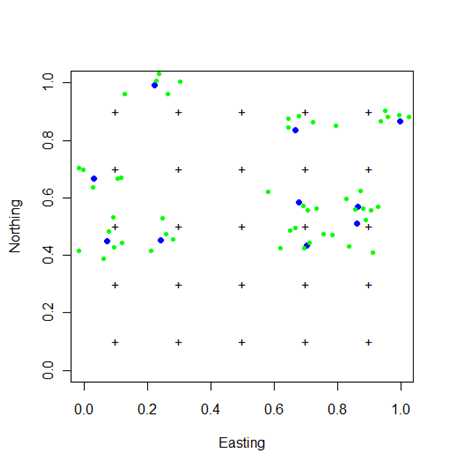
\includegraphics[height=3in]{Ch1/figs/northingeasting}
\end{center}
\caption{Population of $N$ individual home-range centers ($\bf s_i$,
  blue points) and locations during $K=5$ occasions ($\bf u_{ik}$,
  green points). Crosses represent trap locations.}
\label{intro.fig.fig1}
\end{figure}



Although the full model including $u$ and $s$ fully describes the
ecological process, in practice we usually work with reduced forms of
this model. Examples include:
of such models are:
\begin{enumerate}
\item[$\bullet$] Classical distance sampling
\item[$\bullet$] Spatial capture-recapture models with fixed arrays of traps
  \citep{efford:2004, borchers_efford:2008, royle_etal:2009ecol,
    royle_etal:2009jae, gardner_etal:2010ecol,royle_etal:2011jwm}
\item[$\bullet$] Search-encounter models \citep{royle_young:2008, royle_etal:2011mee}.
\item[$\bullet$] Capture-recapture distance-sampling \citep{borchers_etal:1998}.
\end{enumerate}
In some classes of models, components for ${\bf u}$ and ${\bf s}$ will be confounded.
e.g., if ${\bf s}$ are uniform in space and ${\bf u}$ is
a random draw from some distribution centered at ${\bf s}$, then we might as
well define ${\bf u}^{*}=\Pr({\bf u})=\int_{s} [{\bf u}|{\bf s}][{\bf
  s}]ds$ which will itself by uniform
for reasonable choices of $[{\bf u}|{\bf s}]$.  Some examples
of typical spatial capture-recapture models and how
these various model components are manifest in specific cases is
described as follows:
\begin{itemize}
\item[1.] {\bf Distance sampling -- } The last 2 stages of the hierarchy
  are confounded (implicitly) and so analysis is based on the model
  $[y|u*] [u*]$. The ``process model'' is that of ``uniformity'': ${\bf u}^{*}
  \sim Unif({\cal S})$. Sometimes it is argued that distance sampling
  estimators are ``pooling robust'' which is a way of saying they are
  (or may be)
  relatively insensitive to this assumption. That may be true, but the
  construction of distance sampling estimators makes explicit the
  uniformity assumption as a mathematical fact.

\item[2.] {\bf Spatial capture-recapture model with a fixed array of traps} --
SCR models appear to have little in common with distance sampling
because observations are made only at a pre-defined set of discrete
locations -- where traps are placed. However, the models are closely
related in terms of our hierarchical representation above\footnote{Really
they're kind of like point-count distance sampling where the identity
of individuals is preserved across point samples , and distance is a
latent variable. i.e., SCR-DS. I feel like this point should be
emphasized somehow. Here? Later?}
In SCR models based on fixed arrays,
we cannot estimate both
$\Pr(y=1|{\bf u})$ and $\Pr({\bf u}|{\bf s})$ -- the probability  that
an individual ``moves to ${\bf u}$'' cannot be seperated from the
probability that it is detected given that it moves to ${\bf u}$,
because of the fact that the observation locations are fixed by
design.
Formally, such SCR models confound $[y|{\bf u}]$  with $[{\bf
  u}|{\bf s}]$ so that the observation model arises as:
\[
 [y|{\bf s}] = \int_{u} [y|{\bf u}][{\bf u}|{\bf s}] du
\]
This confounding happens because SCR sampling is spatially biased -
restricted to a fixed pre-determined set of locations.

Conversely,
distance sampling confounds $[{\bf u}|{\bf s}][{\bf s}]$ because, essentially, there is
only a single realization of the encounter process.

It is probably
reasonable to assume that $\Pr(y=1|{\bf u})=1$ or at least it is locally
constant for most devices (e.g., cameras, etc..), and thus the
detection model will have the interpretation in terms of movement (see
chapter XXX.YY).

\item[3.] {\bf Search-encounter models -- } What we call
  ``search-encounter'' models \citep{royle_etal:2011mee}
  are kind of a hybrid model - combining features of SCR models and
  features of distance sampling. Like distance sampling they allow for
  encounters in continuous space which provide direct observations
  from $[{\bf u}|{\bf s}]$.
Thus, the
  hierarchical model is fully identified.

\item[4.] {\bf Capture-recapture/distance-sampling -- } See
  \citet{borchers_etal:1998}. As with the search-encounter models the
full hierarchical model is identified:
$[y|{\bf u}][{\bf u}|{\bf s}][{\bf s}]$ but the quantities don't
really mean the same thing as before.

To understand this, we expand the model to accommodate imperfect
measurements of ${\bf u}$. Let ${\bf u}_{obs}$ be an observation of
${\bf u}$ (i.e., made with error). A larger hiearchical model is this:
\[
[y|{\bf u}][{\bf u}_{obs}|{\bf u}][{\bf u}|{\bf s}][{\bf s}]
\]
If we make replicate ``instantaneous'' observations of location, then
information is provided about
 $[{\bf u}_{obs}|{\bf u}]$ (i.e., measurement error). However, in a normal
 distance sampling application, with instantaneous sampling, we don't
 learn anything about $[{\bf u}|{\bf s}]$,
in effect, we are again confounding $[{\bf u}|{\bf s}]$ and $[{\bf
  s}]$: ${\bf u}^{*} = \int_{s} [{\bf u}|{\bf s}][{\bf s}] ds$. So the CR-DS model focuses on:
\[
[y|{\bf u}^{*}][{\bf u}_{obs}|{\bf u}^{*}][{\bf u}^{*}].
\]
Structurally, this is the same basic model as the search-encounter
model notwithstanding (1) that it is usually talked about in terms of
repeated measures of distance instead of location and (2) the 2nd
component of the hierarchy is not movement (an ecological process) but
rather ``measurement error'' and (3) the third component is not a home
range center but rather a movement outcome (``instantaneous
location'').  Thus, while the models are structurally identically, the
meaning and interpretation of quantities are distinct.

%These are
%mostly all semantic and conceptual distinctions which are easy to
%define in a convenient table:
%\begin{table}[ht]
%\centering
%\title{What things mean in each model.}
%\begin{tabular}{c|cc}
%           &   Search encounter models     &  CR-DS  \\  \hline
%  $\sigma$    &  movement       &   measurement error  \\
% ${\bf s}$ & activity center & instaneous location \\
%\end{tabular}
%\end{table}
\end{itemize}


\begin{comment}
\section{Analysis of spatial capture-recapture models}





%\begin{comment}
\subsection{Models don't have political views!}

Whereas hierarchical modeling is a conceptual and framework for
formulating models, the method of inference is independent of model
formulation. Hierarchical models can be analyzed by Bayesian and
non-Bayesian methods. A model is not Bayesian or frequentist -- what
you do to that model is Bayesian or frequentist!
\[
\bullet \mbox{"Hierarchical model"} \ne  \mbox{"Bayesian"}!!!
\]
Thus, analysis of hierarchical models is easily achieved using either
Bayesian or classical (likelihood, frequentist) methods. By
``analysis'' we mean any type of estimation, characterization of
uncertainty, prediction, model selection, or evaluation and we are not
dogmatic about our choice of inference methods. That said, we do
recognize a benefit of the Bayesian approach which is that it
emphasizes model construction and not the construction of
procedures. The Nobel prize\footnote{called something else besides
  Nobel, officially} winning econometrician Christopher Sims (Slides
from the Hotelling Lecture 6/29/2007 at Duke University - cite his
webpage) said it this way: ``Bayesian inference is a way of thinking,
not a basket of 'Methods''' Conversely, ecologistis that are subjected
to a classical statistical curriculum often have only a vague sense of
what the model is that any particular procedure is employing.  We
agree with \citet{little:2006}
that there should be more emphasis on understanding statistical
modeling, and less emphasis on statistical methods.  Toss the ``basket
of methods'' out the window and learn how to model!

%\end{comment}

We rely strictly on principles and procedures of {\it parametric
  inference} in our analysis of hierarchical models in general and,
specifically, of spatial capture-recapture models. Parametric
inference is that in which we make explicit probability assumptions
about how the data were generated. Inference procedures are then
developed under the assumption that the model is truth, because formal
parametric inference procedures that we understand the joint
probability distribution of everything that is a realization of a
random variable. {\bf There is something missing in the previous sentence. require, maybe?}There are two popular flavors of parametric
inference: {\bf Classical inference}: The joint probability distribution
of observations is the {\bf likelihood}. We maximize it to obtain MLEs
and do other fun things to it. We evaluate procedures by thinking
about what would happen over replicate realizations of data to which
our procedures are applied.  {\bf Bayesian inference} is based on the
posterior distribution, which is the joint probability distribution of
the data and also parameters and possibly other quantities including
latent variables or random effects.

Because SCR models contain a collection of latent variables - random
effects -- a natural framework for classical analysis of the models is
based on integrated likelihood \citep{laird_ware:1982,berger_etal:1999}. That is, while
the observation model is conceptualized conditional on the random
effects (the locations of individuals), classical inference is
formally based on the likelihood constructed from the {\it marginal}
probability distribution of the observations (i.e., {\it
  unconditional} on the random effect). The random effects are removed
from the conditional likelihood by integration (which is accomplished
numerically in spatial capture-recapture models). This approach to
inference has been formalized in the context of SCR models by
\citet{borchers_efford:2008, efford:2011}, and implemented for some
classes of models in the software package {\bf DENSITY} \citep{efford:2004}
and the {\bf R} package \mbox{\tt secr} \citep{efford:2011}.

Bayesian analysis is another natural framework for the analysis of
models containing latent variables or random effects.  Under this
approach, analysis of the model is based on Monte Carlo simulation
from the posterior distribution, which is the product of the
conditional likelihood, the distribution of the random effects, and
perhaps other distributions.  This approach was developed by
\citet{royle_young:2008}, and was motivated by work focused on
modeling individual effects in capture-recapture models. In
particular, a convenient reparameterization of individual covariate
models can be obtained using a method known as data augmentation
\citep{royle_etal:2007}, see \citet{royle:2008} for an application to
classical individual covariate models in \citet{royle:2008}. The close
similarity between individual covariate models and spatial
capture-recapture models, with the individual's activity center ${\bf
  s}$ being the individual covariate, led to the application of the
data augmentation method described by \citet{royle_young:2008} and subsequent papers.

These two technical formulations (classical inference based on
integrated likelihood and Bayesian inference) both provide rigorous solutions to
the inference problems posed by spatial capture-recapture data.  There
are also minor distinctions to be aware of. For example,
as a technical matter, \citet{borchers_efford:2008} and related work, assume
a Poisson point process that is unconditional on $N$ whereas Royle and
Young (2008) and related work assume a binomial point process model
which is conditional on $N$.
%More importantly, Borchers and Efford
%develop the analysis in a way that is unconditional on the point
%process (which is removed from the conditional likelihood by
%integration).  Conversely, the analysis of \citet{royle_young:2008} is
%conditional on the underlying point process. As a technical matter,
%Bayesian analysis allows us to analyze the model that is conditional
%on the underlying point process and will otherwise have more
%flexibility - open populations, using telemetry data, etc.. as will be
%demonstrated in later chapters.

We tend to favor Bayesian inference for conceptual and philosphical
reasons but we also think that  integrated likelihood
for complex point process models may prove difficult. On the other
hand, we suspect that Bayesian
analysis by MCMC
of the model that is conditional on the underlying point process will
prove to be more versatile and generalizable for complex point process
models. We say this only
tentatively and throughout this book we are not exclusive in our views
of inference and use Bayesian and classical methods of inference
interchangeable and opportunistically in this book.
We don't want to get too much into the technical foundations of
Bayesian analysis because there are many good books now including
\citet{link_barker:2010}.  \citet{kery:2010, mccarthy:2007,
  king_etal:2009} and probably others by the time this book is
finished. That said,  Bayesian analysis is introduced at a
level required to get through this book in Chapter 2.









\section{Criticisms of Hierarchical Models}

\hl{If we keep this, remove all SCR references b/c Andy will address
  those in Chapt 5}

We have frequently used the terms
``assumptions'' and ``priors'', which make some people feel
uneasy. Our view is that expressed eloquently by Link (ADD
QUOTE). Furthermore, we note that hierarchical models allow us to
modify any assumption deemed too
restrictive. That is, we can always generalize our models given enough
data. Chapter is a classic example because it addresses
perhaps the most common criticism of SCR, that ``real animals'' don't
have symmetic home ranges. In fact people have written entire papers
beating up on SCR because they \emph{assume} that this the bivariate
normal model for the encounter processes is a rigid requirement of SCR
methods. Although we believe this assumption is quite reasonable in
many contexts, Chapter \ref{chapt.ecoldist} clearly illustrates that
alternatives exist, and that SCR provides a rigours framework for
testing for departures from this assumption, and even evaluating
hypotheses that may explain why animals move the way they do.



\end{comment}


